\documentclass{article}
\usepackage{amsthm, amsmath, graphicx, enumitem, tikz-qtree}
\usepackage[margin=1in]{geometry}
\graphicspath{ {6_img/} }
\begin{document}
    \noindent\textbf{CS 373 Homework 6}\hfill Anchu A. Lee\\
    \noindent\today\\
    \begin{enumerate}
        \item Exercise 2.1
            \begin{enumerate}[label =\alph*.]
                \item $E\Rightarrow T \Rightarrow F \Rightarrow a$\\
                    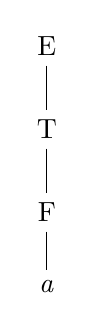
\begin{tikzpicture}[frontier/.style={distance from root=3cm}]
                        \Tree[.E [.T [.F \textit{a} ]]]
                    \end{tikzpicture}
                \item $E \Rightarrow E+T \Rightarrow T+T \Rightarrow F+T \Rightarrow a+T \Rightarrow a+F \Rightarrow a+a$ \\
                    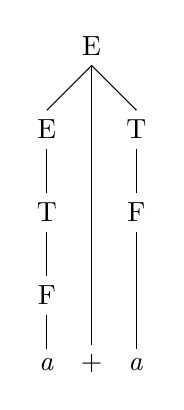
\begin{tikzpicture}[frontier/.style={distance from root=4cm}]
                        \Tree[.E [.E [.T [.F \textit{a} ]]] \text{$+$} [.T [.F \textit{a} ]]]
                    \end{tikzpicture}
                \item $E\Rightarrow E+T \Rightarrow E+T+T \Rightarrow T+T+T \Rightarrow T+T+F \Rightarrow T+F+F \Rightarrow F+F+F \Rightarrow F+F+a
                      \Rightarrow F+a+a \Rightarrow a+a+a$\\
                    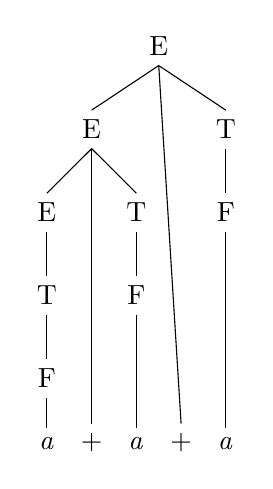
\begin{tikzpicture}[frontier/.style={distance from root=5cm}]
                        \Tree[.E [.E [.E [.T [.F \textit{a} ]]] \text{$+$} [.T [.F \textit{a} ]]] \text{$+$} [.T [.F \textit{a} ]]]
                    \end{tikzpicture}
                \item $E \Rightarrow T \Rightarrow F \Rightarrow (E) \Rightarrow (T) \Rightarrow (F) \Rightarrow ((E)) \Rightarrow ((T)) 
                      \Rightarrow ((F)) \Rightarrow ((a))$\\
                    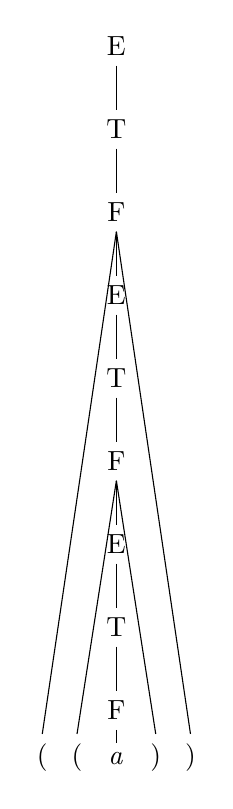
\begin{tikzpicture}[frontier/.style={distance from root=9cm}]
                        \Tree[.E [.T [.F \text{$($} [.E [.T [.F \text{$($} [.E [.T [.F \textit{a} ]]] \text{$)$} ]]] \text{$)$} ]]]
                    \end{tikzpicture}
            \end{enumerate}
        
        \item Construct a pushdown automata that recognizes 
            \begin{center}
                $\{w\mid w \in \{0,1\}^* $ s.t. the number of 0's in $ w $ is equal to the number of 1's in $ w \}$\\
                
                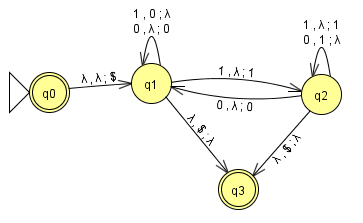
\includegraphics[scale=0.6]{machine1}                
            \end{center}
        \item Exercise 2.2

        \item Exercise 2.4b

        \item Give a CFG for
            \begin{center}
                $\{0^a1^b2^c3^d4^e5^f \mid $ such that $ a,b,c,d,e,f\geq 0 $ and $ a+b=d+e \}$
            \end{center}
        
        \item Exercise 2.4e

        \item Put the rules following in Chomsky normal form (assume that $S$ is the new start variable)
            \begin{align*}
                S&\rightarrow aAA \mid aBC \mid abc\\
                A&\rightarrow AA \mid Aa \mid ab\\
                B&\rightarrow aaBC \mid BC\\
                C&\rightarrow a\mid bc
            \end{align*}
        
        \item Exercise 2.15

        \item Show the following is context free using a CFG
            \begin{center}
                $\{xy \mid x,y\in \{0,1\}^*$, $ |x|=|y|$, $ y\not= x^R\}$
            \end{center}

        \item Construct a pushdown automata that recognizes
            \begin{center}
                $\{w\mid w $ is an element of $\{a,b,c,d\}^* $ such that the number of a's in $w$ plus the number of b's in $w$ is equal to the number of c's in $w$ plus the number of d's in $w \}$
            \end{center}
    \end{enumerate}
\end{document}